\documentclass[10pt, conference]{IEEEtran}
\IEEEoverridecommandlockouts
% The preceding line is only needed to identify funding in the first footnote. If that is unneeded, please comment it out.
\usepackage{cite}
\usepackage{amsmath,amssymb,amsfonts}
\usepackage{algorithmic}
\usepackage{graphicx}
\usepackage{textcomp}
\usepackage{xcolor}
\def\BibTeX{{\rm B\kern-.05em{\sc i\kern-.025em b}\kern-.08em
    T\kern-.1667em\lower.7ex\hbox{E}\kern-.125emX}}
\begin{document}

\title{Selective Regression Testing on Node.js Applications}

\author{\IEEEauthorblockN{Yufeng Chen}
\IEEEauthorblockA{
\textit{University of British Columbia}\\
Vancouver, Canada \\
yufengcy@student.ubc.ca}
}

\maketitle

\begin{abstract}
Node.js is one of the most popular frameworks for building web applications today. As software system 
becomes mature, the cost of performing the retest-all regression test becomes significant. A technique 
of reducing running time is Selective Regression Testing (SRT). By rerunning a subset of tests based on 
code change, selective regression testing can detect software failures more efficiently. However, 
previous studies mainly focused on standard desktop applications. The Node.js applications are 
considered hard to perform test reduction because its asynchronous, event-driven programming model and 
JavaScript is a loosely typed, dynamic programming language. 
In this paper, we present NodeSRT, a Selective Regression Testing framework for Node.js applications. 
By performing static and dynamic analysis, NodeSRT gets relationship between changed method and their 
relationships with each test, then reduce the whole regression test suite to only tests that are 
affected by change, which would improve the execution time of the regression test suite. 
To evaluate our selection technique, we applied NodeSRT to two open-source projects: Uppy and Simorgh, 
then compared our approach with retest-all strategy and current industry used SRT technique: Jest 
OnlyChange option. The results demonstrate that NodeSRT correctly selects affected tests based on 
changes and is 457.94\% more precise than the Jest OnlyChange option. NodeSRT is also 2.72 times faster in 
high code coverage project.
    
\end{abstract}

\begin{IEEEkeywords}
JavaScript, Selective Regression Testing, Node.js Application, Static Analysis, Dynamic Analysis
\end{IEEEkeywords}

\section{Introduction}
With the continuous growth of web applications, Node.js has become one of the most popular frameworks 
for web application development [2]. Since JavaScript is a loosely typed, dynamic language, test 
selection on JavaScript projects is hard. Besides, modern web applications are usually composed of 
different kinds of components; running unit tests only does not judge the overall behaviour of the web 
application [3]. 

Generally, there are two phases involved in test selection. The first phase is to select tests based on change and 
test dependency graph generated by static or dynamic analysis. The second phase is to run selected tests.
There are four levels of granularity for test selection techniques: statement, method, file, module. The common 
two are method-level and file-level. File-level granularity analysis builds relationship between tests and files in 
the program and selects tests that reflect changed files. Method-level analysis builds relationship between tests and methods 
and selects tests that reflect changed method. Since method-level selection is more complicated than 
file-levle selection, file-level selection runs faster in phase one. However, file-level selection selects more 
tests than needed. Therefore it is less precise than method-level selection and runs slower in phase two. 

Current industry used SRT technique: Jest OnlyChange uses file-level granularity, which selects 
tests to be rerun based on file changes in the Git repository. As it is safe and the most light-weighted approach. Although fast, this approach may not be precise 
enough for some test suites. Therefore, our research starts from a question:\textit{"Can we find a more 
effective test selection technique for Node.js Applications?"} 

To evaluate effectiveness of test selection technique, Rothermel et al. [1] proposed four metrics: Inclusiveness, Precision, Efficiency, Generality. Inclusiveness 
measures the extent to which SRT technique chooses tests that are affected by the change. Precision measures 
the ability that SRT technique omits tests that are not affected by the change. Efficiency measures the time and 
space required. Generality measures its ability to function in a comprehensive and practical range of situations.
We say a selection technique is safe if it achieves 100\% inclusiveness.

Our intuition for reducing the total running time is to 
improve the granularity of the selection technique to improve precision so that less tests are required to run in phase two. 
We also evaluated our selection technique by performing an empirical study on two open source Node.js projects in different 
size and code coverage.

\section{Approach Overview}
JavaScript is a dynamic typing, just-in-time compiled, prototype-based object-orientation, multi-paradigm language and supports
event-driven, functional, and imperative programming styles. Many special language features makes tranditional SRT technique
not working on JavaScript programs. These features include first-class functions, Inheritance and the prototype chain, Asynchronous and Error handling. 

To mitigate these challenges, our tool uses a combination of static and dynamic analysis, then perform a modification-based test 
selection algorithm in method level. The Modification-based approach works by analyzing modified code entities 
then select tests based on modifications. This strategy is relatively simple and proved safe by [13] [7]. This tool can 
also be used in CI/CD environment. NodeSRT consists of five parts: dynamic analysis, static analysis, change analysis, 
test selection, and selected test runner. 
\begin{figure}[htbp]
    \centerline{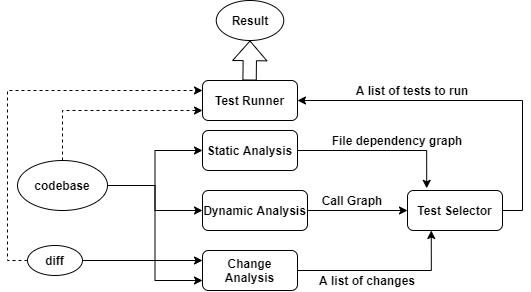
\includegraphics[scale=0.45]{NodeSRT Architecture.png}}
    \caption{NodeSRT Architecture}
    \label{fig}
    \end{figure}    

As shown in Figure 1. The \textbf{Static Analysis module} performs static analysis on original codebase to get file dependency
graph on each tests. It works by identifing and resolving \verb|require| and \verb|import| in JavaScript files. The \textbf{Dynamic Analysis module} generate a dynamic call graph by injecting code to original codebase 
generated AST. Since Node.js applications have the characteristic that client-side, server-side separated, code in 
different modules may be running in a different environment. E.g. The server-side code is running in Node.js 
environment. Client-side code is running in the browser environment. To collect runtime information of each 
module, NodeSRT uses HTTP requests. The injected code will send logging messages to the server. The logging server will 
collect all the logging messages and generate a call graph in JSON format. As noted by [13][14], when the codebase 
becomes large, code analysis result should be store in database to ensure performance. \textbf{Change Analysis module} 
compares the ASTs of the changed files, then generate a JSON representation of changes. Since NodeSRT uses function-level 
granularity, change analysis module finds the closest function name of each different AST node based on their ancestors. 
If the function is anonymous, NodeSRT will generate a unique name for it based on its parent function name, class name and file name. 
This approach is similar to the approach of Chianti [16] handling anonymous class in Java. With call graph, file dependency graph, 
and JSON representation of changes, \textbf{Test Selector} selects tests affected by changes. To handle changes outside 
functions, the test selector will select tests depend on the changed file based on file dependency graph to guarantee safety. 
Finally, The \textbf{Test Runner} will run selected tests.

Our tool can also be used to select end-to-end tests since NodeSRT uses HTTP requests 
record logging messages and build dynamic call graph.

\section{Empirical Evaluation}

\section{Related Work}
% this paragraph might need refactoring.
There are several techniques proposed for standard desktop applications [1, 6, 7, 9, 10, 11, 13, 14, 15, 16], 
not much study focused on Node.js web applications. For JavaScript projects, Mutandis [19] is a generic mutation testing 
approach that guides the mutation generation process. It works by leveraging static and dynamic program 
analysis to guide the mutation generation process a-priori towards parts of the code that are error-prone or 
likely to influence the program’s output. 
Tochal [20] is a DOM-Sensitive change impact analysis tool for JavaScript. Through dynamic code injection and static analysis, this 
approach incorporates a ranking algorithm for indicating the importance of each entity in the impact set. This 
approach focused on frontend DOM changes, rather than the whole frontend backend interaction.

For test selection in different levels of granularity, Gligoric et al. [4] showed that file-level granularity 
analysis runs 32\% faster than the method-level granularity analysis in large scale Java programs.  [12] also shows 
tool implemented with approach "DejaVu" [11] is 16\% worse when it comes to realistic code-coverage-based test suites.
This is becuase there are two phases required for SRT. The first step is to select tests based on change and 
test dependency graph generated by static or dynamic analysis. The second phase is to run selected tests. For 
some project, if the running time of selecting tests plus the running time of executing selected tests is 
greater than the running time of executing the whole test suite, applying the selection technique is 
meaningless. This is the reason of current industry used approach only use file-level granularity static analysis as this is the 
most light-weight, simple approach. 

\section{Prepare Your Paper Before Styling}
Before you begin to format your paper, first write and save the content as a 
separate text file. Complete all content and organizational editing before 
formatting. Please note sections \ref{AA}--\ref{SCM} below for more information on 
proofreading, spelling and grammar.

Keep your text and graphic files separate until after the text has been 
formatted and styled. Do not number text heads---{\LaTeX} will do that 
for you.

\subsection{Abbreviations and Acronyms}\label{AA}
Define abbreviations and acronyms the first time they are used in the text, 
even after they have been defined in the abstract. Abbreviations such as 
IEEE, SI, MKS, CGS, ac, dc, and rms do not have to be defined. Do not use 
abbreviations in the title or heads unless they are unavoidable.

\subsection{Units}
\begin{itemize}
\item Use either SI (MKS) or CGS as primary units. (SI units are encouraged.) English units may be used as secondary units (in parentheses). An exception would be the use of English units as identifiers in trade, such as ``3.5-inch disk drive''.
\item Avoid combining SI and CGS units, such as current in amperes and magnetic field in oersteds. This often leads to confusion because equations do not balance dimensionally. If you must use mixed units, clearly state the units for each quantity that you use in an equation.
\item Do not mix complete spellings and abbreviations of units: ``Wb/m\textsuperscript{2}'' or ``webers per square meter'', not ``webers/m\textsuperscript{2}''. Spell out units when they appear in text: ``. . . a few henries'', not ``. . . a few H''.
\item Use a zero before decimal points: ``0.25'', not ``.25''. Use ``cm\textsuperscript{3}'', not ``cc''.
\end{itemize}

\subsection{Equations}
Number equations consecutively. To make your 
equations more compact, you may use the solidus (~/~), the exp function, or 
appropriate exponents. Italicize Roman symbols for quantities and variables, 
but not Greek symbols. Use a long dash rather than a hyphen for a minus 
sign. Punctuate equations with commas or periods when they are part of a 
sentence, as in:
\begin{equation}
a+b=\gamma\label{eq}
\end{equation}

Be sure that the 
symbols in your equation have been defined before or immediately following 
the equation. Use ``\eqref{eq}'', not ``Eq.~\eqref{eq}'' or ``equation \eqref{eq}'', except at 
the beginning of a sentence: ``Equation \eqref{eq} is . . .''

\subsection{\LaTeX-Specific Advice}

Please use ``soft'' (e.g., \verb|\eqref{Eq}|) cross references instead
of ``hard'' references (e.g., \verb|(1)|). That will make it possible
to combine sections, add equations, or change the order of figures or
citations without having to go through the file line by line.

Please don't use the \verb|{eqnarray}| equation environment. Use
\verb|{align}| or \verb|{IEEEeqnarray}| instead. The \verb|{eqnarray}|
environment leaves unsightly spaces around relation symbols.

Please note that the \verb|{subequations}| environment in {\LaTeX}
will increment the main equation counter even when there are no
equation numbers displayed. If you forget that, you might write an
article in which the equation numbers skip from (17) to (20), causing
the copy editors to wonder if you've discovered a new method of
counting.

{\BibTeX} does not work by magic. It doesn't get the bibliographic
data from thin air but from .bib files. If you use {\BibTeX} to produce a
bibliography you must send the .bib files. 

{\LaTeX} can't read your mind. If you assign the same label to a
subsubsection and a table, you might find that Table I has been cross
referenced as Table IV-B3. 

{\LaTeX} does not have precognitive abilities. If you put a
\verb|\label| command before the command that updates the counter it's
supposed to be using, the label will pick up the last counter to be
cross referenced instead. In particular, a \verb|\label| command
should not go before the caption of a figure or a table.

Do not use \verb|\nonumber| inside the \verb|{array}| environment. It
will not stop equation numbers inside \verb|{array}| (there won't be
any anyway) and it might stop a wanted equation number in the
surrounding equation.

\subsection{Some Common Mistakes}\label{SCM}
\begin{itemize}
\item The word ``data'' is plural, not singular.
\item The subscript for the permeability of vacuum $\mu_{0}$, and other common scientific constants, is zero with subscript formatting, not a lowercase letter ``o''.
\item In American English, commas, semicolons, periods, question and exclamation marks are located within quotation marks only when a complete thought or name is cited, such as a title or full quotation. When quotation marks are used, instead of a bold or italic typeface, to highlight a word or phrase, punctuation should appear outside of the quotation marks. A parenthetical phrase or statement at the end of a sentence is punctuated outside of the closing parenthesis (like this). (A parenthetical sentence is punctuated within the parentheses.)
\item A graph within a graph is an ``inset'', not an ``insert''. The word alternatively is preferred to the word ``alternately'' (unless you really mean something that alternates).
\item Do not use the word ``essentially'' to mean ``approximately'' or ``effectively''.
\item In your paper title, if the words ``that uses'' can accurately replace the word ``using'', capitalize the ``u''; if not, keep using lower-cased.
\item Be aware of the different meanings of the homophones ``affect'' and ``effect'', ``complement'' and ``compliment'', ``discreet'' and ``discrete'', ``principal'' and ``principle''.
\item Do not confuse ``imply'' and ``infer''.
\item The prefix ``non'' is not a word; it should be joined to the word it modifies, usually without a hyphen.
\item There is no period after the ``et'' in the Latin abbreviation ``et al.''.
\item The abbreviation ``i.e.'' means ``that is'', and the abbreviation ``e.g.'' means ``for example''.
\end{itemize}
An excellent style manual for science writers is \cite{b7}.

\subsection{Authors and Affiliations}
\textbf{The class file is designed for, but not limited to, six authors.} A 
minimum of one author is required for all conference articles. Author names 
should be listed starting from left to right and then moving down to the 
next line. This is the author sequence that will be used in future citations 
and by indexing services. Names should not be listed in columns nor group by 
affiliation. Please keep your affiliations as succinct as possible (for 
example, do not differentiate among departments of the same organization).

\subsection{Identify the Headings}
Headings, or heads, are organizational devices that guide the reader through 
your paper. There are two types: component heads and text heads.

Component heads identify the different components of your paper and are not 
topically subordinate to each other. Examples include Acknowledgments and 
References and, for these, the correct style to use is ``Heading 5''. Use 
``figure caption'' for your Figure captions, and ``table head'' for your 
table title. Run-in heads, such as ``Abstract'', will require you to apply a 
style (in this case, italic) in addition to the style provided by the drop 
down menu to differentiate the head from the text.

Text heads organize the topics on a relational, hierarchical basis. For 
example, the paper title is the primary text head because all subsequent 
material relates and elaborates on this one topic. If there are two or more 
sub-topics, the next level head (uppercase Roman numerals) should be used 
and, conversely, if there are not at least two sub-topics, then no subheads 
should be introduced.

\subsection{Figures and Tables}
\paragraph{Positioning Figures and Tables} Place figures and tables at the top and 
bottom of columns. Avoid placing them in the middle of columns. Large 
figures and tables may span across both columns. Figure captions should be 
below the figures; table heads should appear above the tables. Insert 
figures and tables after they are cited in the text. Use the abbreviation 
``Fig.~\ref{fig}'', even at the beginning of a sentence.

\begin{table}[htbp]
\caption{Table Type Styles}
\begin{center}
\begin{tabular}{|c|c|c|c|}
\hline
\textbf{Table}&\multicolumn{3}{|c|}{\textbf{Table Column Head}} \\
\cline{2-4} 
\textbf{Head} & \textbf{\textit{Table column subhead}}& \textbf{\textit{Subhead}}& \textbf{\textit{Subhead}} \\
\hline
copy& More table copy$^{\mathrm{a}}$& &  \\
\hline
\multicolumn{4}{l}{$^{\mathrm{a}}$Sample of a Table footnote.}
\end{tabular}
\label{tab1}
\end{center}
\end{table}

\begin{figure}[htbp]
\centerline{
\includegraphics{fig1.png}}
\caption{Example of a figure caption.}
\label{fig}
\end{figure}

Figure Labels: Use 8 point Times New Roman for Figure labels. Use words 
rather than symbols or abbreviations when writing Figure axis labels to 
avoid confusing the reader. As an example, write the quantity 
``Magnetization'', or ``Magnetization, M'', not just ``M''. If including 
units in the label, present them within parentheses. Do not label axes only 
with units. In the example, write ``Magnetization (A/m)'' or ``Magnetization 
\{A[m(1)]\}'', not just ``A/m''. Do not label axes with a ratio of 
quantities and units. For example, write ``Temperature (K)'', not 
``Temperature/K''.

\section*{Acknowledgment}

The preferred spelling of the word ``acknowledgment'' in America is without 
an ``e'' after the ``g''. Avoid the stilted expression ``one of us (R. B. 
G.) thanks $\ldots$''. Instead, try ``R. B. G. thanks$\ldots$''. Put sponsor 
acknowledgments in the unnumbered footnote on the first page.

\section*{References}

Please number citations consecutively within brackets \cite{b1}. The 
sentence punctuation follows the bracket \cite{b2}. Refer simply to the reference 
number, as in \cite{b3}---do not use ``Ref. \cite{b3}'' or ``reference \cite{b3}'' except at 
the beginning of a sentence: ``Reference \cite{b3} was the first $\ldots$''

Number footnotes separately in superscripts. Place the actual footnote at 
the bottom of the column in which it was cited. Do not put footnotes in the 
abstract or reference list. Use letters for table footnotes.

Unless there are six authors or more give all authors' names; do not use 
``et al.''. Papers that have not been published, even if they have been 
submitted for publication, should be cited as ``unpublished'' \cite{b4}. Papers 
that have been accepted for publication should be cited as ``in press'' \cite{b5}. 
Capitalize only the first word in a paper title, except for proper nouns and 
element symbols.

For papers published in translation journals, please give the English 
citation first, followed by the original foreign-language citation \cite{b6}.

\begin{thebibliography}{00}
\bibitem{b1} G. Eason, B. Noble, and I. N. Sneddon, ``On certain integrals of Lipschitz-Hankel type involving products of Bessel functions,'' Phil. Trans. Roy. Soc. London, vol. A247, pp. 529--551, April 1955.
\bibitem{b2} J. Clerk Maxwell, A Treatise on Electricity and Magnetism, 3rd ed., vol. 2. Oxford: Clarendon, 1892, pp.68--73.
\bibitem{b3} I. S. Jacobs and C. P. Bean, ``Fine particles, thin films and exchange anisotropy,'' in Magnetism, vol. III, G. T. Rado and H. Suhl, Eds. New York: Academic, 1963, pp. 271--350.
\bibitem{b4} K. Elissa, ``Title of paper if known,'' unpublished.
\bibitem{b5} R. Nicole, ``Title of paper with only first word capitalized,'' J. Name Stand. Abbrev., in press.
\bibitem{b6} Y. Yorozu, M. Hirano, K. Oka, and Y. Tagawa, ``Electron spectroscopy studies on magneto-optical media and plastic substrate interface,'' IEEE Transl. J. Magn. Japan, vol. 2, pp. 740--741, August 1987 [Digests 9th Annual Conf. Magnetics Japan, p. 301, 1982].
\bibitem{b7} M. Young, The Technical Writer's Handbook. Mill Valley, CA: University Science, 1989.
\end{thebibliography}
\vspace{12pt}

\end{document}
